%!TEX root = ../document.tex
\chapter{Implementation}\label{ch:implemenation}

\begin{quotation}
"Tiny modules built on other tiny modules to make tiny powerful high level abstractions".
{\small\it -- James Halliday (substack), founder of browserling, prolific Node.js developer}
\end{quotation}

During the process of developing browserCloud.js, several attempts were created following the Agile methodology, rapidly creating working prototypes and iterating over them. This led to the creation of several open source modules, MIT licensed, having been downloaded in the order of dozens of thousand times until the creation of this document.

Every code artifact was developed following the Unix philosophy, every module attempts to do at most one thing and one thing well, creating small, maintainable and powerful abstractions.

In this section, we describe the implementation details of the final code artifacts that compose the browserCloud.js and the collaterals designed and created that although not projected in the beginning, were needed in order to collect the data we were looking to study.

\section{Browser module}

The browser module is the agent that sits inside our browser nodes, implementing all the communication protocols designed for the browserCloud.js platform and exposing a developer API to send and receive messages.

Essentially it is broken down into 4 components:

\begin{itemize}
    \item channel manager - a code artefact responsible to levarage the websockets connection with the signalling server and abstracts the necessary work to open new RTCPeerConnections with other peers.
    \item finger table manager - where the information about a specific peer finger table lives.
    \item router - the routing logic to deliver the messages on the most efficient way. It uses finger table manager to understand what is the most efficient way.
    \item interface - developer exposed interface.
\end{itemize}

\begin{figure}[h!]
  \centering
  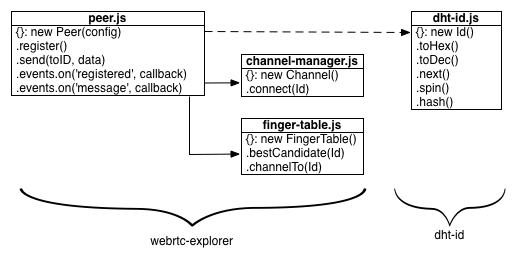
\includegraphics[width=0.7\textwidth]{figs/diagram-webrtc-explorer}
  \caption{Code Structure of webrtc-explorer, the JavaScript module that implements the client code for browserCloudjs}
  \label{fig:d-w-e}
\end{figure}

The browser module exposes a factory method, meanthing that a developer can instantiate several instances inside a browser. The code for this module is structured as indicated by Figure~\ref{fig:d-w-e} and Figure~\ref{fig:d-w-e-b-p}. We can see that the Job Scheduler (webrtc-explorer-browser-process), is an service developed on top of base browser module (webrtc-explorer).

\begin{figure}[h!]
  \centering
  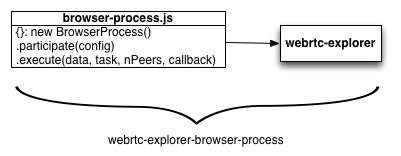
\includegraphics[width=0.7\textwidth]{figs/diagram-webrtc-explorer-browser-process}
  \caption{Code Structure of the abstraction on top of webrtc-explorer to compute parallel tasks over the browser network}
  \label{fig:d-w-e-b-p}
\end{figure}



There are two technologies used in this module, other than the raw Javascript APIs that the browser offers, these are:

\begin{itemize}
    \item browserify - enables the development of browser Javascript code in a modular fashion using the CommonJS standard, such as Node.js does, this means we can require('modules') and create concat and minify our Browser module, so that it can be loaded inside a webpage through a normal <script> tag.
    \item socket.io - socket.io is the most reliable and famous open source implementation of WebSocket API for the browser..
\end{itemize}

\section{Signalling server}

The signalling server offers two Web APIs, one being a WebSockets API and the other a RESTful API. The design decision behind these two APIs was mainly because since the network evolves with time, we needed a way to be able to push, on demand, new information to browsers, for example, when a new peer needs to be railed in, or when the Signalling Server acts as a rendezvous point for SDP data exchange between browsers so they can establish a RTCPeerConnection. Figure~\ref{fig:d-s-s} shows the Code Structure for this application.

\begin{figure}[h!]
  \centering
  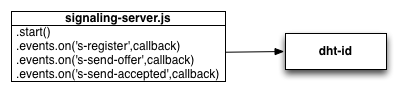
\includegraphics[width=0.6\textwidth]{figs/diagram-signalling-server}
  \caption{Code Structure of the Signalling Server}
  \label{fig:d-s-s}
\end{figure}

The second API, RESTful, is used to instruct the server or to collect analytics data from it remotely.

\section{Key learnings from the earlier iterations - webrtc-ring}

During one of the earlier iterations, we've developed a prototype of webrtc-explorer, called webrtc-ring, which although very similiar in routing strategy, each peer only knew about its successor, in another words, each peer only had access to one finger, this originated a system with the following properties:

\begin{itemize}
    \item overlay structure - 1 dimension Hash Ring
    \item lookup protocol - Matching key and NodeID
    \item network parameters - Number of Nodes in the network
    \item routing table size - 1
    \item routing complexity - O(log(N))
    \item join/leave overhead - 2
\end{itemize}

During the development, we performed tests to evaluate the capacity of the system to distribute work, later discussed on the Evaluation section. We learned that due to the single thread nature of Javascript, running message routing inside the same process that would be use to perform CPU bound tasks could be highly disavantageous for browserCloud.js performance. To overcome this, we introduced Web Workers to the system, independent threads inside the browser to separate communication from CPU bound tasks.

\section{Testing framework - piri-piri}

Figure~\ref{fig:d-p-p}

\begin{figure}[h!]
  \centering
  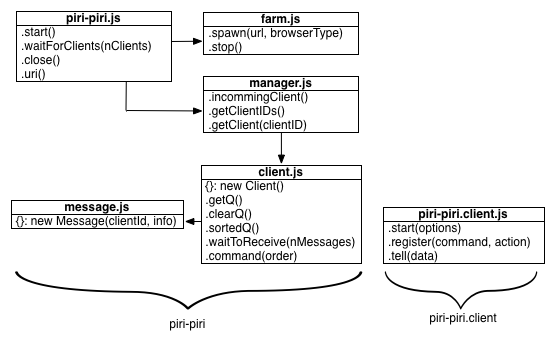
\includegraphics[width=0.7\textwidth]{figs/diagram-piri-piri}
  \caption{Code Structure for the Testing Framework, named piri-piri}
  \label{fig:d-p-p}
\end{figure}

explain here how things work (class diagrams and such)

\section{Visualize the network state}

Using D3JS, a API library that works as a thin veneer on top of SVG, we've developed an application that grabs the state of the browserCloud.js network and shows a live graphical representation, as seen on Figure~\ref{fig:visualizer}, where each node is represented by a dot and its ID and the arcs being the connections established between the nodes in the network .Figure~\ref{fig:d-v} shows the Code Structure for this application.

\begin{figure}[h!]
  \centering
  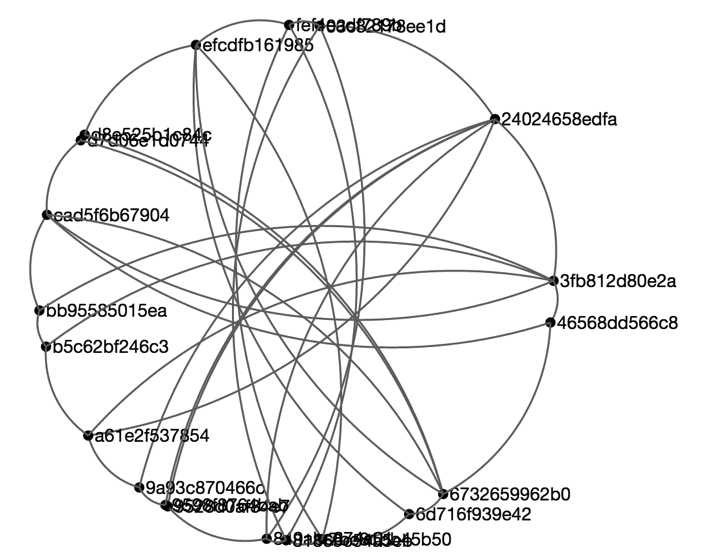
\includegraphics[width=0.7\textwidth]{figs/visualizer}
  \caption{Visualization of a browserCloud.js network}
  \label{fig:visualizer}
\end{figure}

\begin{figure}[h!]
  \centering
  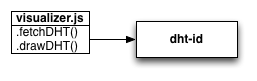
\includegraphics[width=0.4\textwidth]{figs/diagram-visualizer}
  \caption{Code Structure for the Visualizer application}
  \label{fig:d-v}
\end{figure}

\section{Simulate a browserCloud.js network}

In addition to the visualizer application, one simulator application was developed, were not only a graphical representation is generated, but also, it gives the developer a way to create a new virtual network, without any real peers. We've the option to pick the number of peers we want present and how many and which fingers will be used, so we can analyse different distribution paths and optimize for number of hops between any two peers in the network. Figure~\ref{fig:d-s} shows the Code Structure for this application.


\begin{figure}[h!]
  \centering
  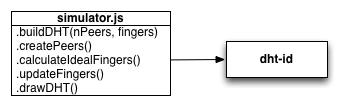
\includegraphics[width=0.4\textwidth]{figs/diagram-simulator}
  \caption{Code Structure for the Simulator application}
  \label{fig:d-s}
\end{figure}

\section{Ray Tracing module}

To perform the parallel CPU bound tests, we've developed a module that works in Node.js and in the browser to perform Ray Tracing Tasks. The module works in a synchronous fashion so it performs faster, in another words, there are not techniques to make que module asynchronous that would create an overhead for the processing, in order to avoid stopping javascript event loop, the ray tracing task has to be ran in a sub process.

This module performs the interpretation of a scene designed in CSS, division of the scene in multiple parts (tasks) and reconstruction of the ray traced scene when every task is completed. We can observe in Figure~\ref{fig:d-s-r}, how this module is structured

\begin{figure}[h!]
  \centering
  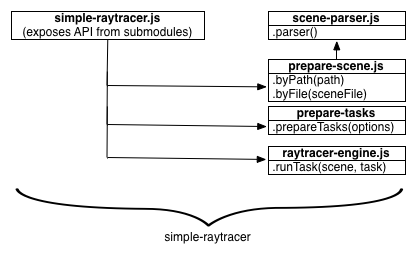
\includegraphics[width=0.6\textwidth]{figs/diagram-simple-raytracer}
  \caption{Code Structure for the Ray Tracing module}
  \label{fig:d-s-r}
\end{figure}

\section{Summary}

SO MUCH CODE
